\section{Overview}
\label{sec:overv}

In this section, we will give a brief introduction on how our application functions.

\subsection{Pipeline Overview}

\begin{figure}
    \centering
    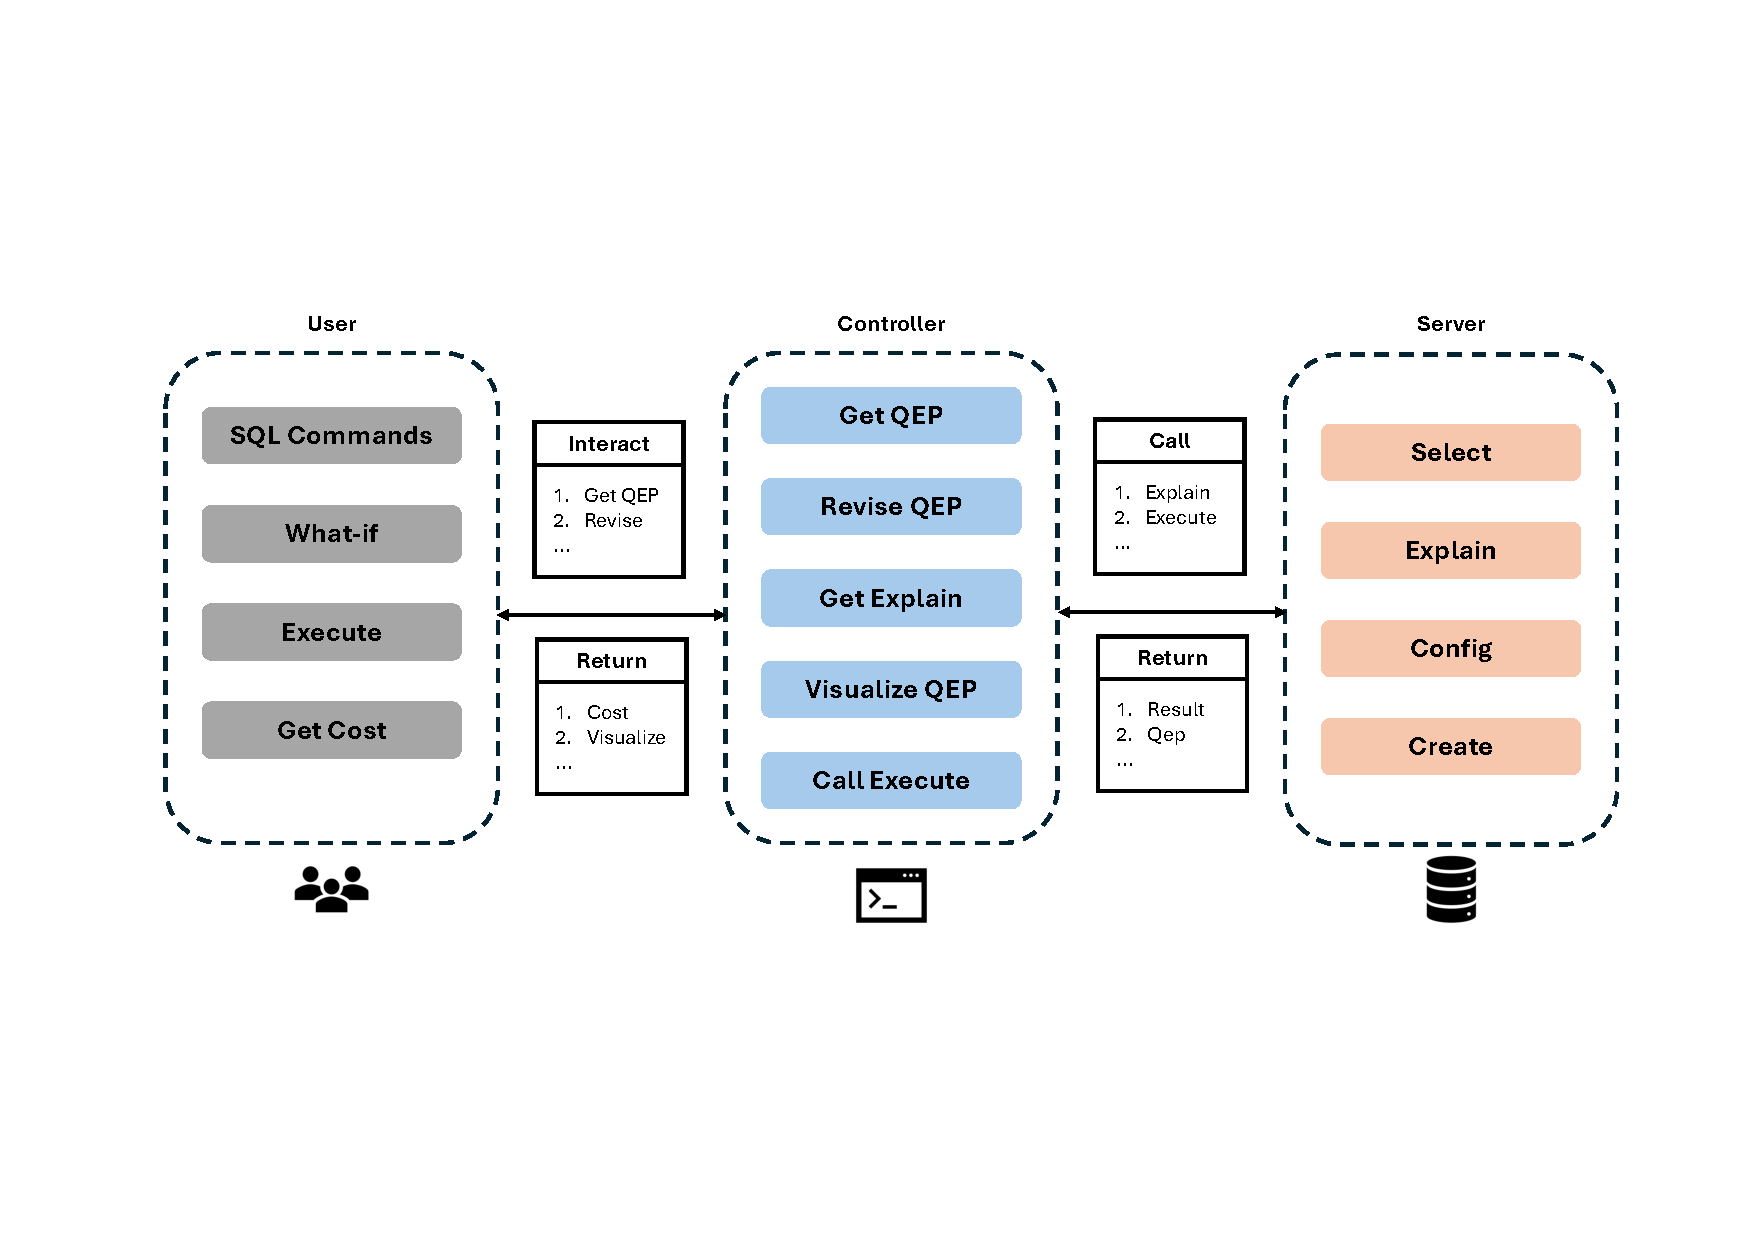
\includegraphics[width=1\linewidth]{figures/Pipeline.pdf}
    \caption{A overview of our pipeline. Where user can perform different operations and receive results from the controller and the server side. The user can freely decide when to execute the commands}
    \label{fig:pipeline}
\end{figure}

Our application mainly consist of three key components: \textbf{1)} A user-interface to allow user to interact with. \textbf{2)} A controller component that post the commands to the server and get the result. \textbf{3)} A database server that actually execute the commands and store the data.

Our application follows a modular pipeline that integrates a backend for query processing and a frontend for user interaction. The pipeline consists of several stages:

\paragraph{Database Connection} Users first connect to the PostgreSQL database through the GUI by providing connection details. If necessary, they can load a prepared dataset from the Internet and create the corresponding table in the database. This operation is performed only once and stores the \textit{tpch} dataset on the server.

\paragraph{Query Plan Retrieval} Users can input SQL queries or select examples through the GUI. Once a valid command is entered in the code panel, the QEP visualization is displayed. The execution and retrieval process algorithm is implemented efficiently, providing real-time details on costs, explanations, and tree visualizations. Further details about the algorithm are available in~\cref{sec:algo}.

\paragraph{Interactive What-If Analysis} Users can modify the query execution plan by changing join types or scan methods through the GUI. A list of options is provided, and changes are reflected in real time in the cost estimation and tree visualization. Planner settings are dynamically adjusted using SQL commands (e.g., \texttt{SET enable\_*}) based on the query planning configuration. Details of the algorithm are provided in~\cref{subsec:whatif-algo}.

\paragraph{Visualization and Explanation} After retrieving the QEP or the revised AQP from the server, the system parses it into a tree where each node represents an operation and its condition. This parsed tree is used to calculate the coordinates of the visualized QEP tree. We also provide natural language explanations derived from the tree using a post-order traversal. Each step is parsed according to a set of predefined rules and formats, then presented to the user.

\paragraph{Comparison and Results} Once the user is satisfied with their query plan, they can execute it to view the actual query results and query log. The system displays the query execution time, enabling users to validate performance.

\subsection{Application Structure}

The application is organized into the following key components:

\paragraph{Frontend} Gradio~\cite{abid2019gradio} is used as our frontend framework. The GUI accepts user inputs (connection details, SQL queries, and what-if modifications) and displays query plans, costs results and logs to the user. It also provides interactive dropdown menus for what-if analysis.

\paragraph{Backend} We adopted FastAPI~\cite{fastapi} as the framework to provide the backend server logic. The backend contacts the database in SQL commands, with Psycopg 3.

\paragraph{Database System} PostgreSQL~\citep{postgres_github} is selected as the Database system to manage our database. The database is established from TPC-H dataset~\cite{poess2000new}.\footnote{Version 3.0.1, retrieved from \href{https://www.tpc.org/TPC_Documents_Current_Versions/download_programs/tools-download-request5.asp?bm_type=TPC-H&bm_vers=3.0.1}{this link}, compiled with \texttt{Visual Studio 2022 version 17.10}.} To make it easier to reproduce our experiments on different devices, we have uploaded the data to Hugging Face Datasets~\cite{lhoest2021datasets}, which could be accessed by \href{https://huggingface.co/datasets/pufanyi/TPC-H}{this link}.

% \paragraph{Controllers of our system}
% \begin{enumerate}
%     \item  \textbf{Frontend (User Interface)}
%     \begin{itemize} 
%     \item Framework: Gradio~\cite{abid2019gradio} for GUI development.
%     \item Responsibilities: \begin{itemize} 
%     \item Accept user inputs (connection details, SQL queries, and what-if modifications).
%     \item Display query plans, costs, results, and logs.
%     \item Provide interactive dropdown menus for what-if analysis.
% \end{itemize}
%     \item Files: 
%     \begin{itemize}
%         \item \textit{interface.py}: Implements the Gradio GUI with components for database connection, query input, query plan visualization, and cost comparison. 
%         \item Other static files such as css, js, and html file for the base url
%     \end{itemize}  
% \end{itemize}


%     \item  \textbf{Backend (Query Processing)}
%     \begin{itemize} 
%     \item Framework: FastAPI~\citep{fastapi} for backend server logic.
%     \item Responsibilities: \begin{itemize} 
%     \item Establish database connections and manage \textit{TPC-H}~\cite{poess2000new} data.
%     \item Process user modifications to join and scan methods.
%     \item Pass SQL commands to PostgreSQL and retrieve results from PostgreSQL.
%     \item Provide APIs for the frontend to fetch query plans and costs.
% \end{itemize}
%     \item Files: \begin{itemize} 
%     \item \textit{project.py}: Main script for launching the server and handling CLI arguments.
%     \item \textit{whatif.py}: Contains algorithms for generating SQL commands based on user-selected join and scan methods.
%     \item \textit{tcph.py}: Contains the controller to interact with the database server.
%     \item \textit{ExecutionTree.py}: Contains all the code to parse the query plan into a tree.
%     \item \textit{visualizer.py}: Contains all the code to visualize the Execution Tree.
% \end{itemize}    

% \end{itemize}

%     \item  \textbf{Database}
%     \begin{itemize} 
%     \item System: PostgreSQL~\citep{postgres_github} with the \textit{TPCH} dataset.
%     \item Responsibilities: \begin{itemize} 
%     \item Execute SQL queries and provide query execution plans (QEPs).
%     \item Support advanced planner configurations for what-if analysis.
% \end{itemize}

% \end{itemize}

% \end{enumerate}

\subsection{Key Interaction Flow}

\paragraph{Database Connection} User connects to the database via GUI $\to$ FastAPI establishes the connection $\to$ PostgreSQL confirms the connection $\to$ Download the dataset from Hugging Face $\to$ Load data to the database.

\paragraph{Query Execution} User inputs query $\to$ Gradio sends request to FastAPI $\to$ FastAPI receives the query and send to PostgreSQL $\to$ PostgreSQL generates QEP and computes results and costs, then returns them to the FrontEnd.

\paragraph{What-If Analysis} User modifies join/scan types on the FrontEnd $\to$ Gradio sends modification request $\to$ FastAPI adjusts planner settings and send to PostgreSQL $\to$ PostgreSQL generates AQP and estimated costs.

\paragraph{Result Display} Results, costs, explains and logs are visualized in the GUI.
